\documentclass[a4paper]{article}
\usepackage{graphicx}
\usepackage{xcolor}
\usepackage{url}
\usepackage{outlines}
\usepackage{listings}
\usepackage{fontspec}
\lstset{basicstyle=\ttfamily,
	showstringspaces=false,
	commentstyle=\color{blue},
	keywordstyle=\color{pink}
}
\lstset{emph={
	EXPOSE,RUN,FROM,CMD,nc,tcp,udp,http,docker},emphstyle=\color{purple}
}
\newcommand{\abc}{\hfill \break}
\usepackage{fancyhdr}
\usepackage{geometry}
\geometry{
	a4paper,
	total={170mm,257mm},
	left=20mm,
	top=20mm,
	bottom=39mm,
}

\setlength{\headheight}{82.70538pt}

\fancypagestyle{oida}{
	\fancyhf{}
	\fancyhead[L]{\fontsize{7.5}{7.5}htl donaustadt\\ Donaustadtstraße 45\\
		1220 Wien\\~\\ Abteilung: Informationstechnologie\\ 
	Schwerpunkt: Netzwerktechnik}
	\fancyhead[R]{
\includegraphics[scale=0.45]{images/logo.png}}

	\fancyfoot[L]{\today}
	\fancyfoot[C]{\jobname}
	\fancyfoot[R]{Seite: \thepage}
}

\begin{document}
\bibliographystyle{plain}
\pagestyle{oida}
\section*{GNU/Linux - Securing access}
\par\noindent\rule{\textwidth}{0.4pt}

Laboratory protocol

\begin{figure}[h]
	
\includegraphics[scale=0.3]{images/mika.jpeg}
	\caption{Grouplogo}
\end{figure}

\vspace*{\fill}
Subject:	ITSI|ZIVK

Class:	3AHITN

Name:	Stefan Fürst, Marcel Raichle

Gruppenname/Nummer: Dumm und Dümmer/7

Supervisor: 	ZIVK

Exercise dates:

Submission date:


\newpage
\tableofcontents

\newpage

\section{Task definition}



\section{Summary}


\newpage

\section{Exercise Execution}

%give better title
\subsection{Privileged rights}
\subsubsection{Explanation of the sudo command}
The \texttt{sudo} command or \textbf{S}uper\textbf{U}ser \textbf{DO} temporarily elevates privileges and runs the set command as root, which can be seen by running the \texttt{sudo id} command.\cite{sudo}

\begin{figure}[h]
	\centering
	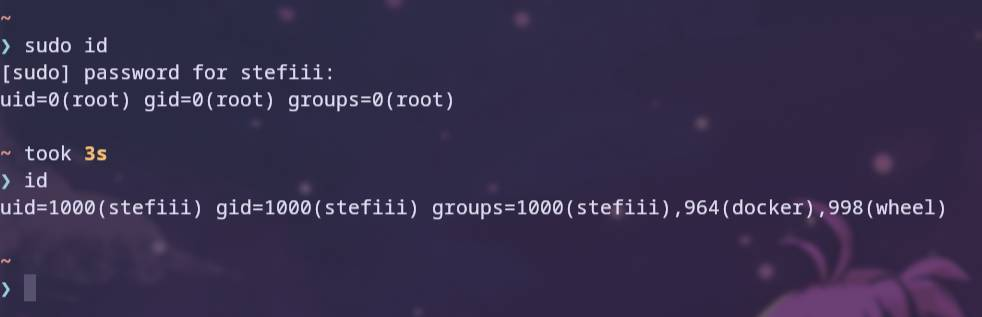
\includegraphics[scale=0.4]{images/sudoid.png}
	\caption{sudo id}
\end{figure} \abc
As seen in the figure, when the \texttt{id} command is used with \texttt{sudo}, the id displayed is 0, which is the user id of the root user, and without sudo it displays the normal user id of the user who executed the command.

\subsubsection{Granting and restricting users' sudo access}
To grant someone permission to run any command with \texttt{sudo}, the \texttt{usermod -aG sudo username} command is used, which appends the given to the sudo group, giving them permission to run any command with sudo. \abc
In order to restrict the commands that can be elevated by a user or to configure other settings related to this, it is necessary to edit the configuration file, which is located at \texttt{/etc/sudoers}.\abc
There are several ways to edit it. The \texttt{visudo} command uses the editor set in the \texttt{\$EDITOR} environment variable and opens the sudoers file with it, and when you exit the editor and save it, it also checks for errors before applying the changes.
The sudoers file can also be directly edited using \texttt{echo} in the dockerfile.
\begin{lstlisting}[language=bash]
#only allowing ram-alois to edit the ssh configuration file
RUN echo "ram-alois ALL=(root) /bin/nano /etc/ssh/sshd_config" >> /etc/sudoers
#only allowing ram-berta to add users
RUN echo "ram-berta ALL=(root) /sbin/useradd" >> /etc/sudoers
#only allowing to ram-ram to view and read add files
RUN echo "ram-ram ALL=(root) /bin/ls" >> /etc/sudoers
RUN echo "ram-ram ALL=(root) /bin/cat" >> /etc/sudoers
\end{lstlisting}
I chose nano over vim for editing the ssh config file, as running vim as sudo effectively gives the user full sudo access, as it is possible to open a terminal in it and escape the normal editor mode in numerous ways, so its just easier to give the user nano.\abc
insert screenshots of the thing
\newpage
\subsubsection{Setting up a password policy}
To set password policies on Debian-based distrobutions, edit \texttt{/etc/pam.d/common-password}. Pam stands for Pluggable Authentication Modules and is installed by default on every Debian-based distribution.\cite{password-policies-1}\cite{password-policies-2} \abc
To set a required complexity for passwords, the \texttt{libpam-pwquality} package needs to be installed. Then in the \texttt{/etc/pam.d/common-password} file, on the line with \texttt{pam\_pwquality.so} \texttt{dcredit=-1}, \texttt{ocredit=-1} and \texttt{enforce\_for\_root} need to be added at the end to require at least one lowercase letter and one symbol in any password set and to enforce it for the root user.\abc
Preventing password reuse is achieved by adding a line with the \texttt{pam\_pwhistory.so} module and appending \texttt{remember=5} and \texttt{use\_authtok} at the end of the line to remember the last 5 passwords so that they cannot be reused and to enforce the previously stacked password modules.\cite{password-policies-2}
Finally, set the minimum length of the line with \texttt{pam\_unix.so}. \texttt{minlen=10} to require the password to be at least 10 characters long. \abc
To edit this file declaratively in the Dockerfile I used the \texttt{sed} editor and the sed commands used are explained in the next section.
\begin{lstlisting}[language=bash]
#setting the requied password complexity
RUN sed -i '/retry=3/ s/$/ucredit=-1 dcredit=-1 ocredit=-1/ enforce_for_root'\
            /etc/pam.d/common-password
#remebering the last 5 passwords so they cant be reused
RUN sed -i '/dit=-1/ a password\trequisite\t\t\tpam_pwhistory.so remember=5 use_authtok'\
            /etc/pam.d/common-password
#setting the minimum length
RUN sed -i '/yescrypt/ s/$/ minlen=10/' /etc/pam.d/common-password
\end{lstlisting}
\subsubsection{sed Basics}
todo explain sed

\newpage
\section{References}
\bibliography{quellen}
\newpage
\section{List of figures}

\listoffigures

\end{document}
